\chapter{Proposed LTE-R Test-bed Implementation and Results}
\label{chapter4}

This chapter provides background information on LTE proposed for high-speed railway communication system. It outlines the architecture for LTE-R leveraging the existing LTE network for high speed railway networks. For uniform coverage inside a tunnel environment, leaky coaxial cables (LCX) has been proposed for efficient communication. We explain LCX cables in details in the following chapter especially for tunnel environment. The severe channel impairments inside a tunnel are also discussed with special attention to high Doppler shift cause due to high velocities of trains and harsh multipath fading environment. Finally, the proposed two-ray propagation channel model is discussed and dynamic K-factor is derived.

\section{LTE-R Testbed in Matlab}

We have implemented the simulation testbed in MATLAB, consisting of a transmitter, a channel and a receiver. The K-factor values for the channel model are obtained from Eq.(\ref{kfactor}) and are used to generate a time-series BER curve for different modulation schemes used in LTE-R. The values used for the electrical material properties for tunnel walls~\cite{lter17} and its
specifications are given in Table~\ref{tablelter}. The relative permittivity for the tunnel walls is taken as $\varepsilon_r = 5$ and $\sigma$ is set to 0.1. The simulation is conducted for velocity of $v (Km/h) = $ 300, 400 and 500 Km/h. Since the frequency band allocation for LTE-R will most probably be from 2--6 GHz, hence the $f_c$ values chose are 2, 3 and 5 GHz. The height of the receiver is assumed to be around the length of the train and height of tunnel is chosen as the size of the leaky coaxial cable.

\begin{table*}[t!]
\centering
\caption{Tunnel and Tx/Rx Characteristics}
\begin{tabular}{c  c  c }
   & Dimensions & Simulation Parameters\\\hline
Tunnel & Width = 8.6 m, Height = 7.3 m & $\varepsilon_r = 5$, $\sigma = 0.1~\textrm{Sm}^{-1}$\\\hline
Leaky Feeder Cable (Tx) & Height = 6.1 m & $f_c$ (GHz) = 2, 3, 5\\\hline
Train (Rx) & Height = 4.2 m &  v (km/h) = 300, 400, 500\\
\hline
\end{tabular}
\label{tablelter}
\end{table*}

\begin{figure}[!ht]
\label{finalblock}
\centering
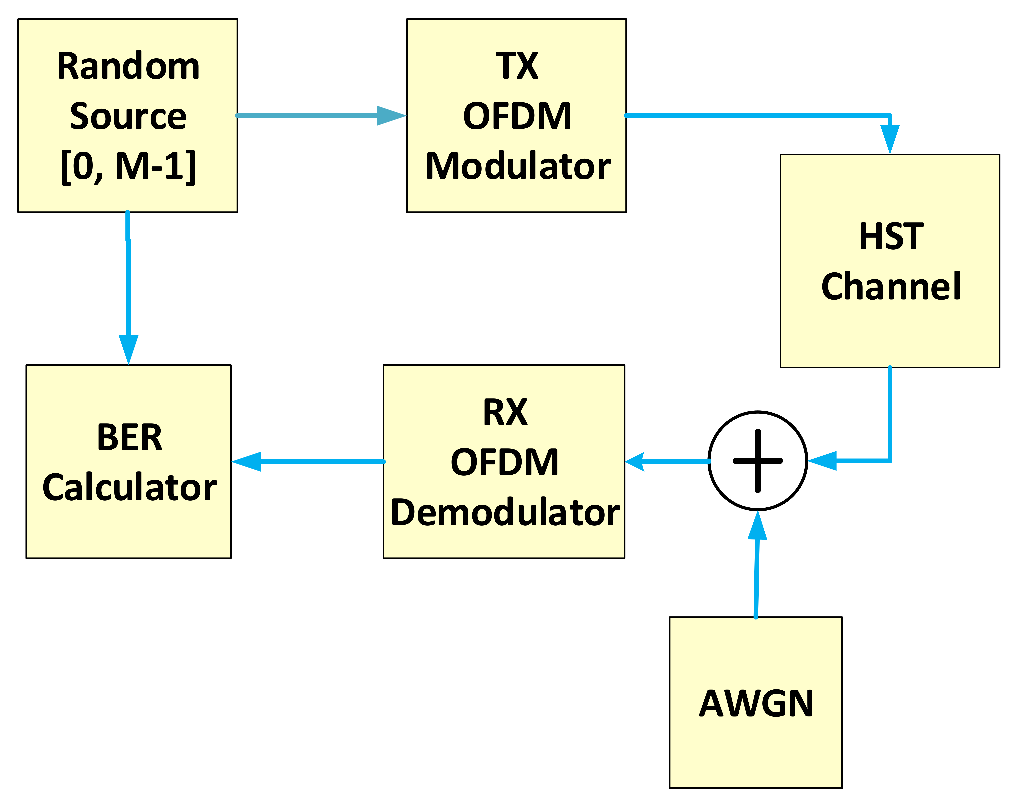
\includegraphics[width=\textwidth,height=8cm,keepaspectratio]{images/Gill/lte_figs/finalblock.eps} 
\caption{Block diagram of a communication system through a HST channel using QPSK, 16-QAM and 64-QAM.}
\end{figure}

Figure~\ref{finalblock} shows the block diagram of the simulation test-bed used for the performance analysis of LTE-R. The random source block generate the symbol between 0 and M-1, where M = 4,16,64 for QPSK, 16QAM and 64QAM respectively. The data is then modulated with specific modulation type and then pass through the proposed HST channel model. The additive white gaussian noise is added after applying the channel coefficients to the signal data. We then demodulate the data packets and pass it to the ber calculator object which then computes the bit-error rate. The simulations are run for SNR values ranging from 0--20 dB and plots are generated for all three modulation schemes.

\section{HST LTE-R in a Tunnel}
Using LTE System Toolbox provided by MATLAB we generated Figure~\ref{lteofdma} which shows the received resource grid without equalization. The frame worth of data was modulated with QPSK, 16QAM and 64QAM for equal number of subcarriers and mapped to symbol in a subframe. We generate ten subframes individually and create one frame after merging all subframes. The frame is passed through our proposed high speed train channel model, with additive white gaussian noise added. We can see that without equalization the received resourced grid has lot of errrors and will lead to numerous retransmissions.

\begin{figure}[!ht]
\label{lteofdma}
\centering
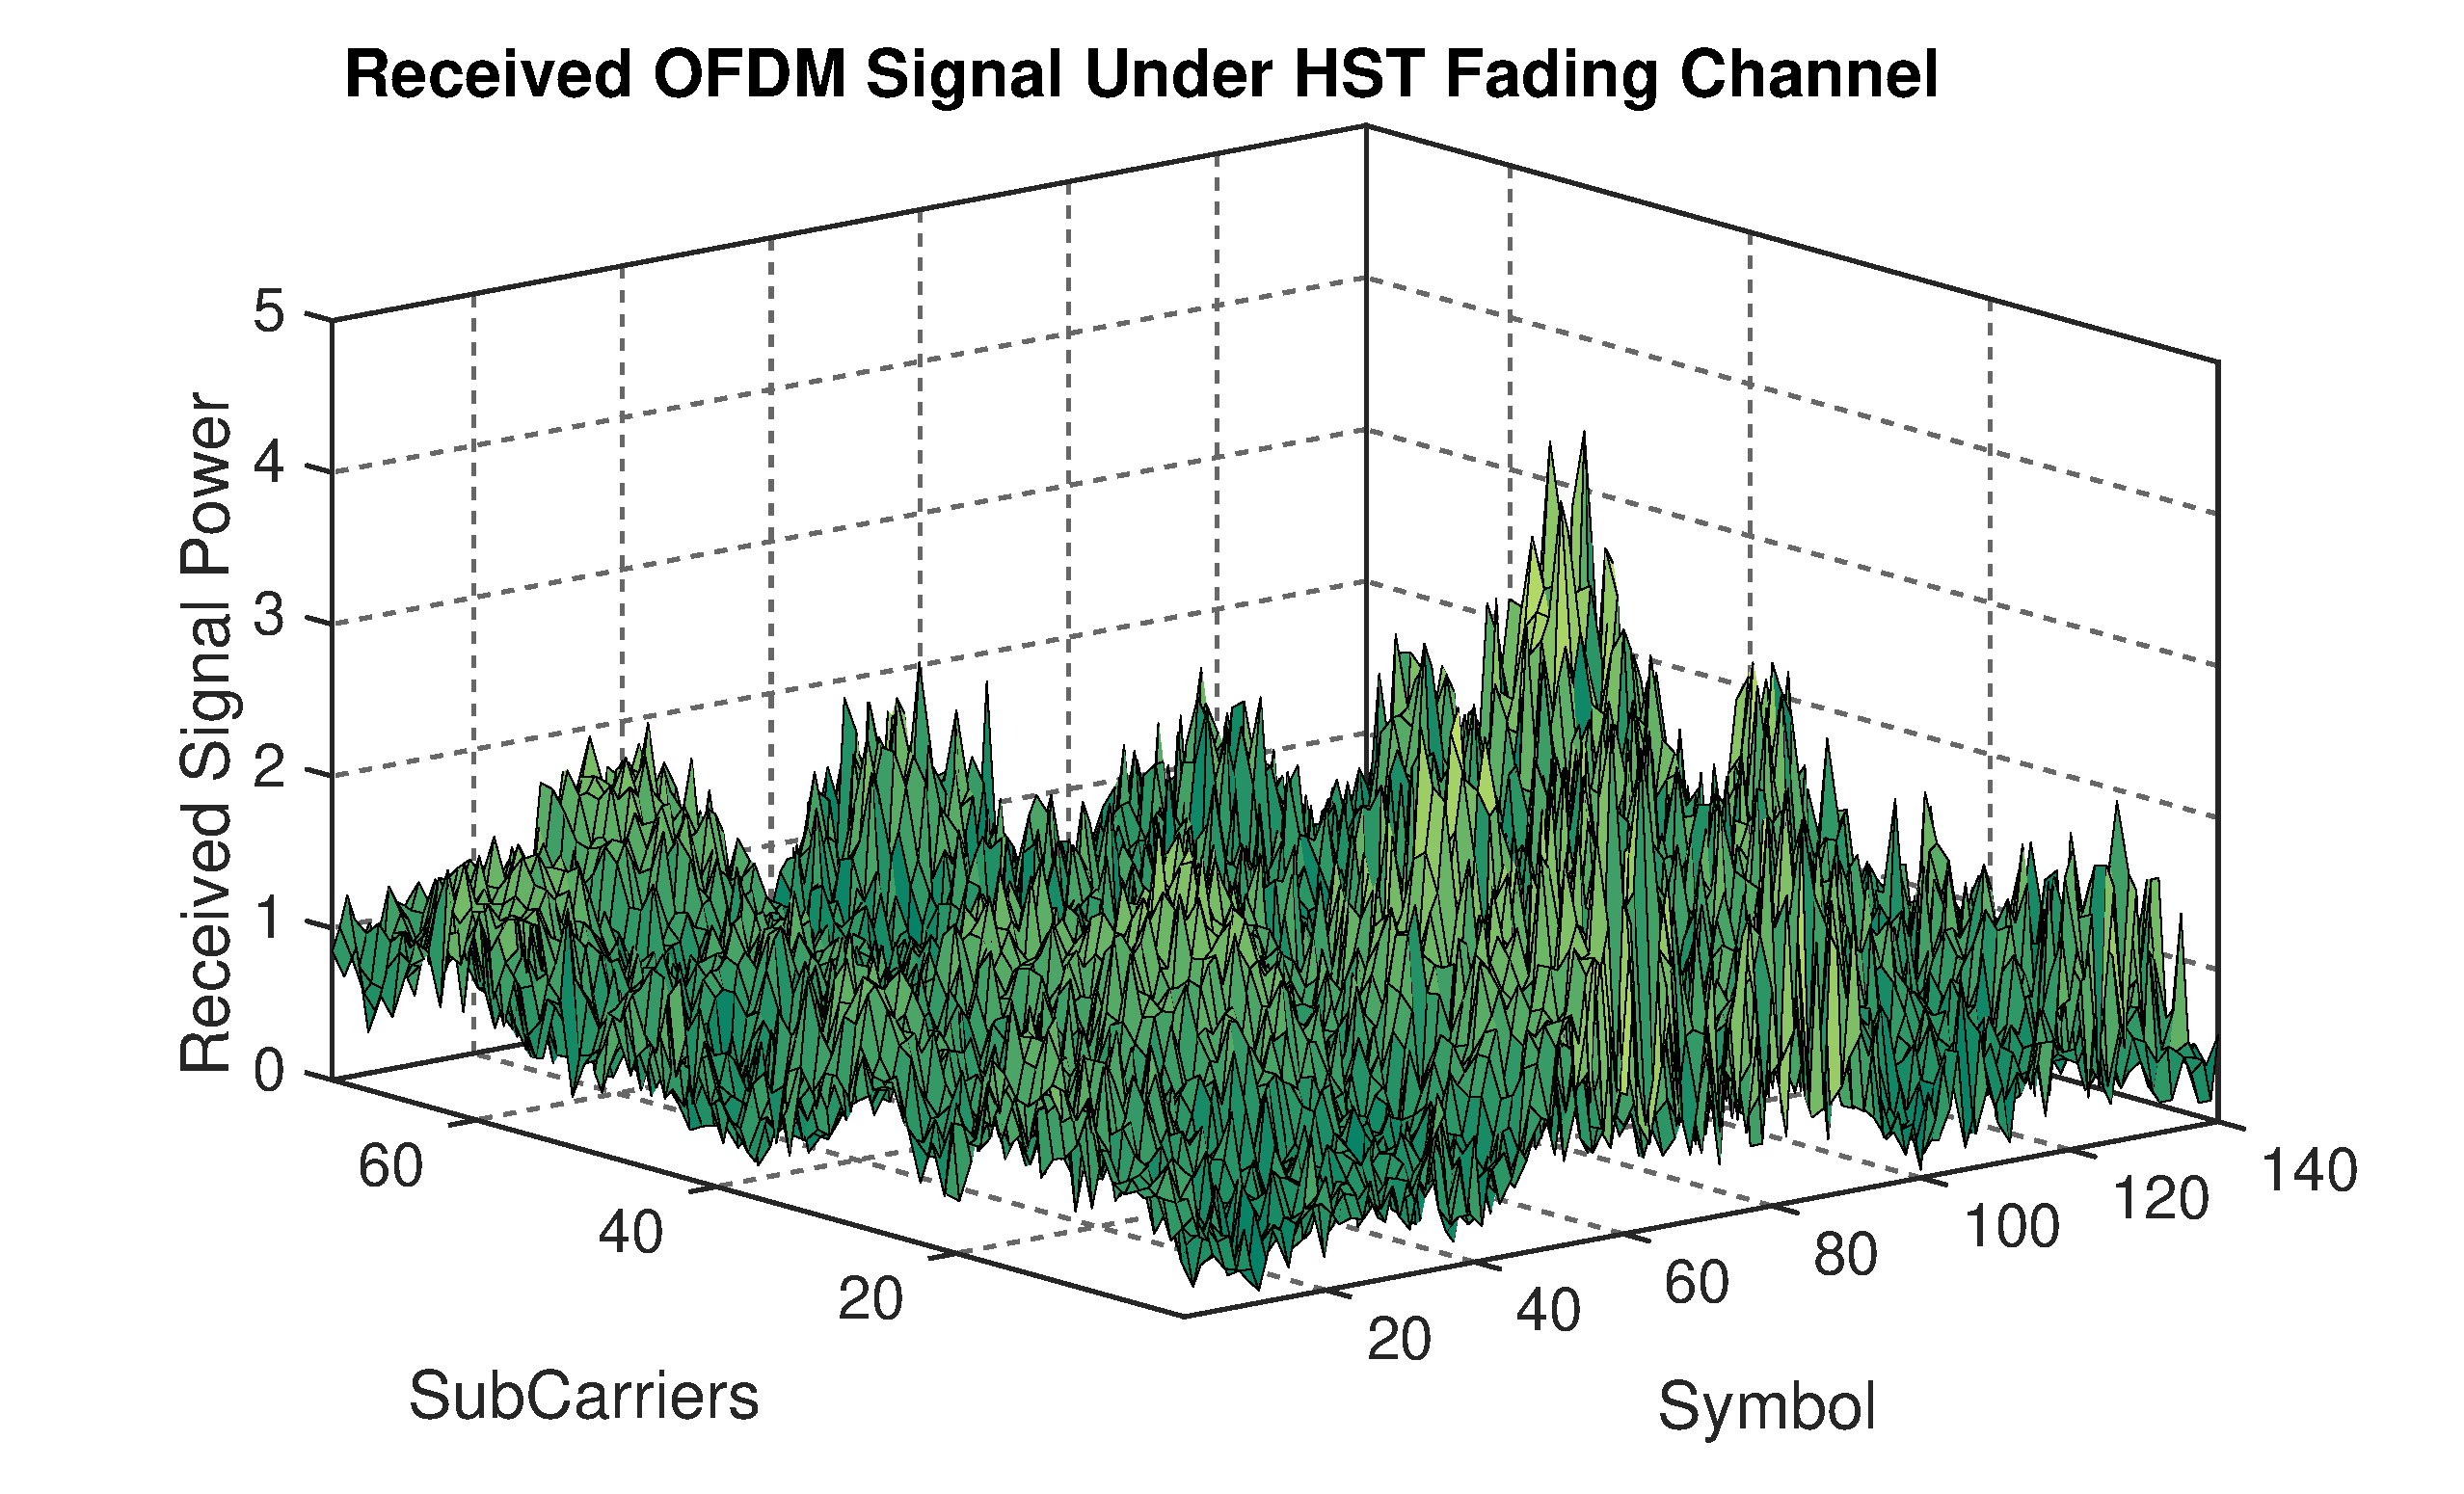
\includegraphics[width=\textwidth,keepaspectratio]{images/Gill/lte_figs/receivedsignal.eps} 
\caption{Received LTE-R OFDM signal under HST Ricean Fading Environment. }
\end{figure}

\subsection{K-factor in a Tunnel}
In Figure~\ref{kfactorber}, we calculated the K-factor for the HST inside a tunnel with velocity $v$ = 500 km/h for different center frequencies. It shows the variation of the Rician K-factor with the distance between the transmitter and receiver as the train is moving along the tunnel. We computed the K-factor for a leaky cable with periodic slots separated by distance d in fixed time-steps. The plot shows that the K-factor varies significantly over a short distances. Therefore, assuming a single K-factor for the channel model is not accurate, we use time-series K-factor to do our channel modeling.

\begin{figure}[!ht]
\label{kfactor}
\centering
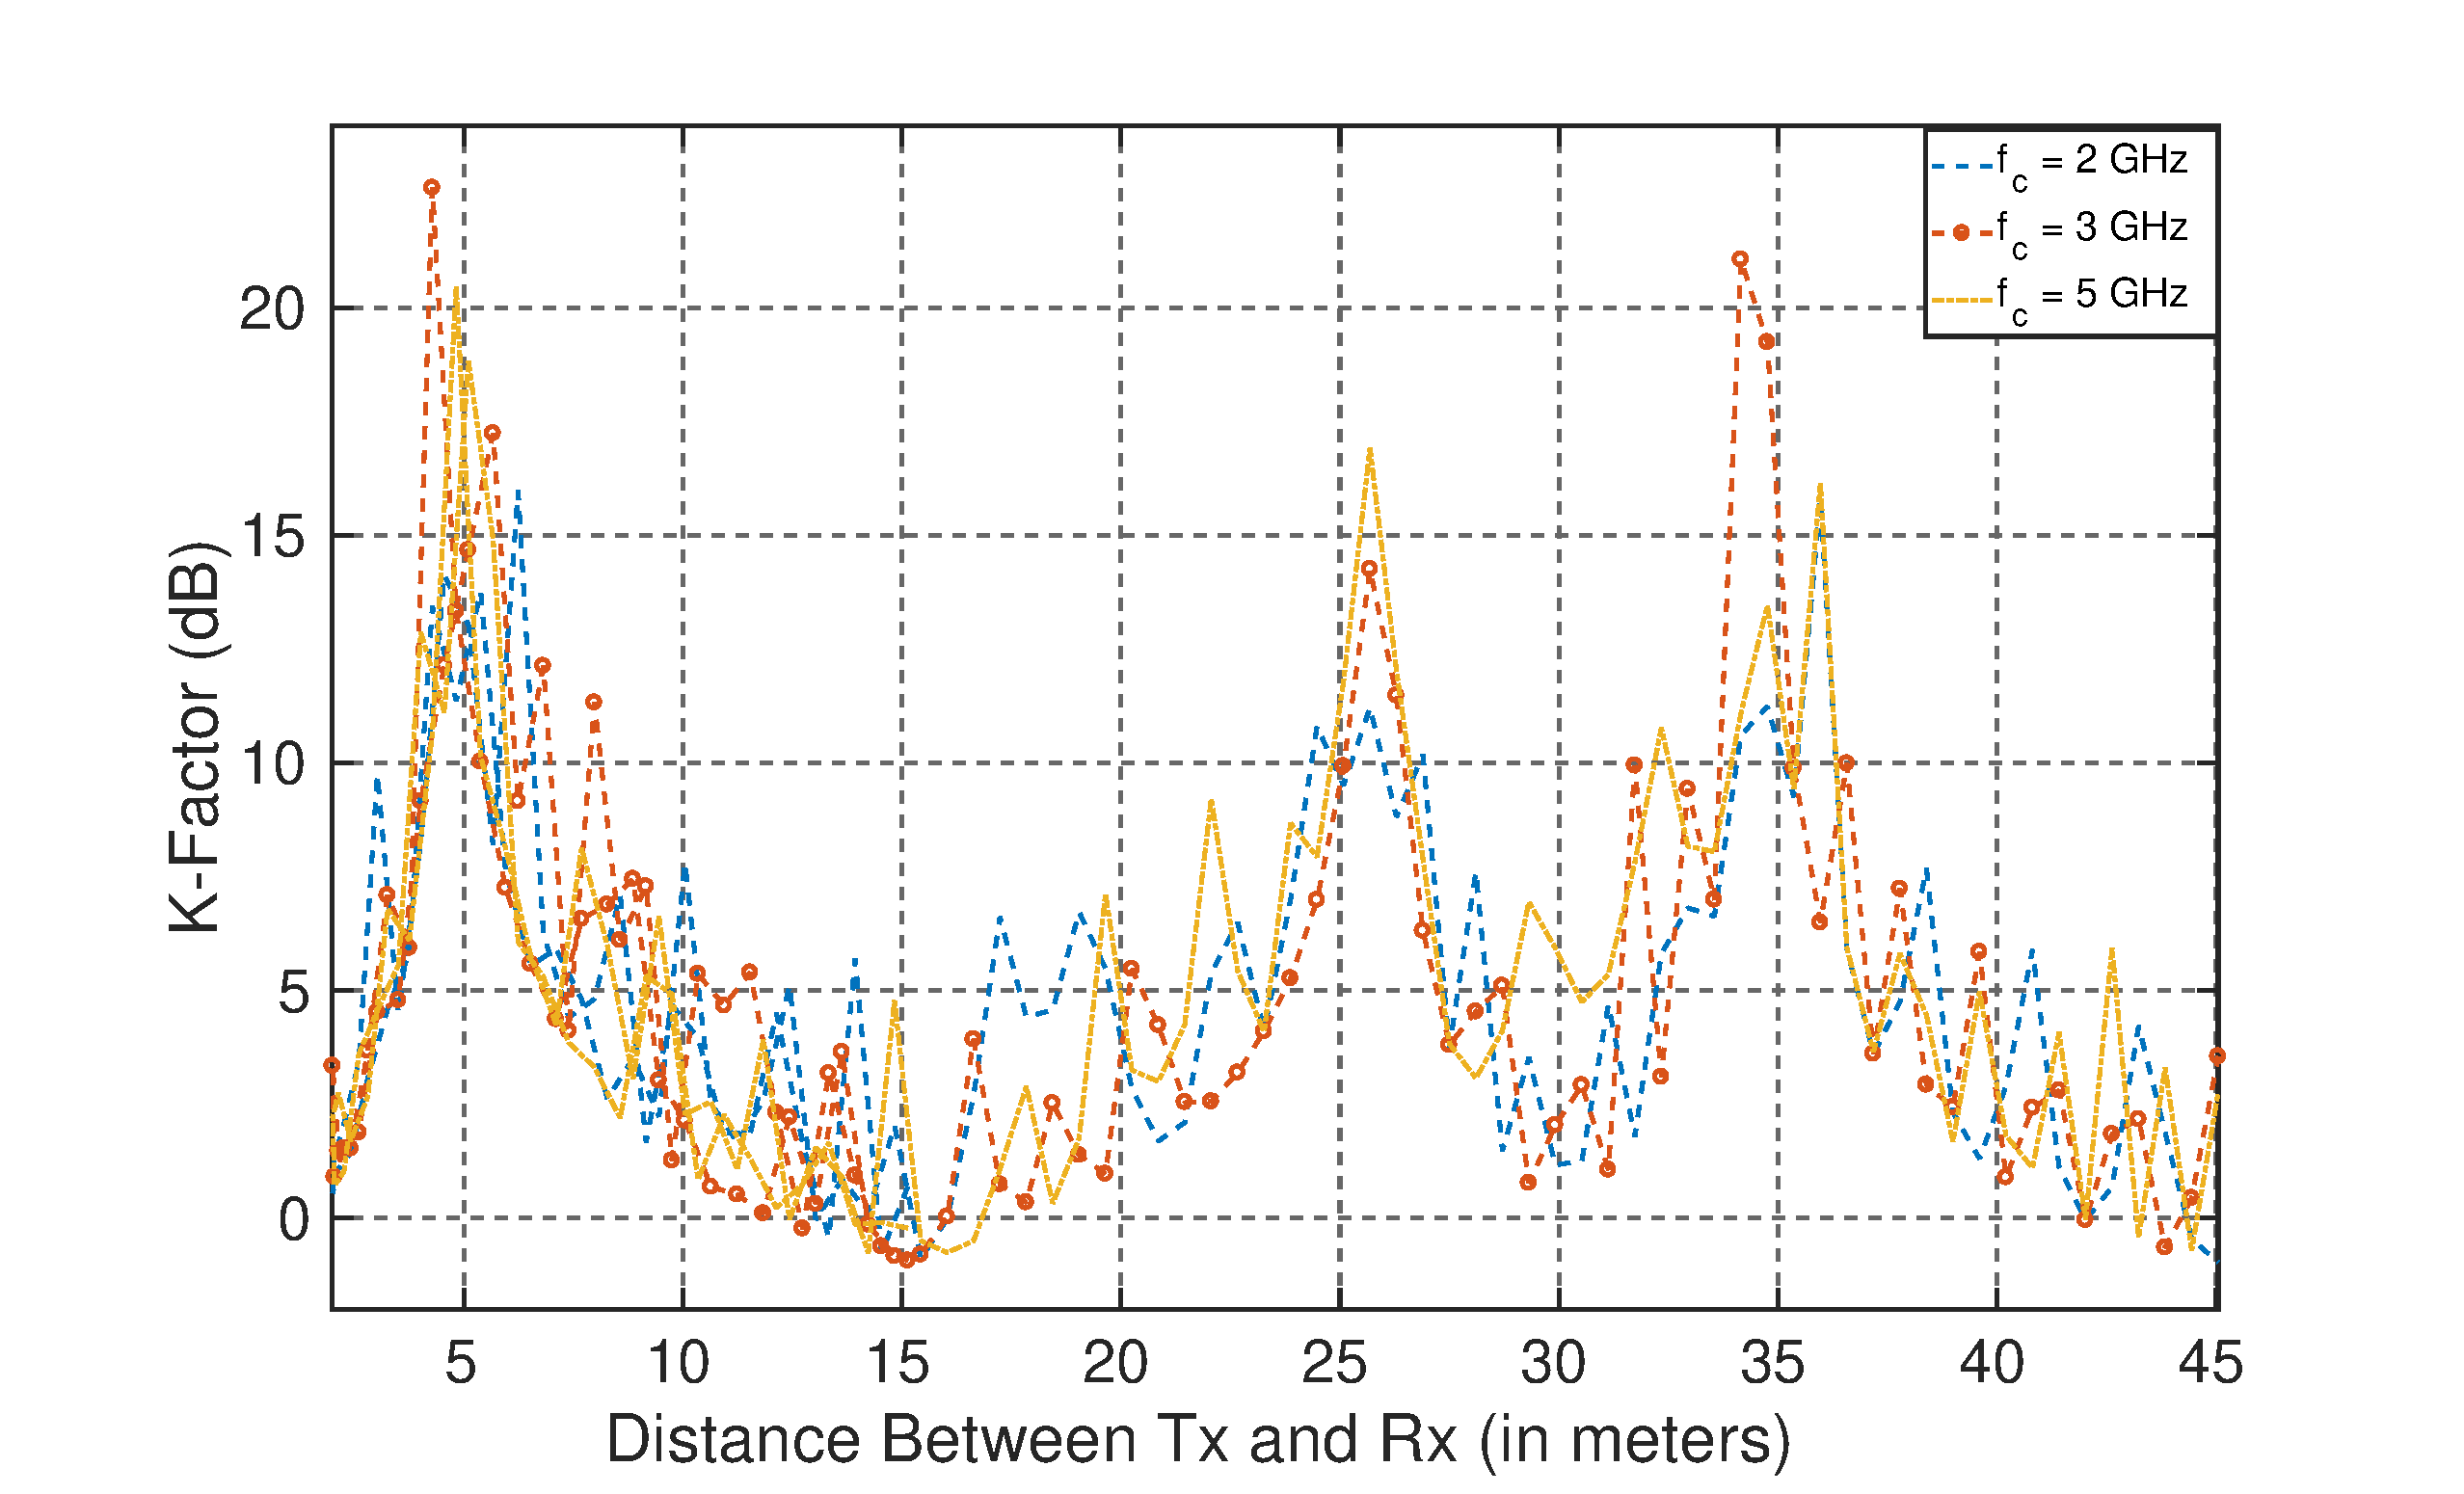
\includegraphics[width=\textwidth,keepaspectratio,height=8cm]{images/Gill/lte_figs/kfactordist.eps} 
\caption{K-factor versus $D_{LOS}$ for different center frequencies $f_c$ = 2, 3 and 5 GHz.}
\end{figure}

\subsection{BER Performance}
To show the impact of varying K-factor on the channel, we computed the BER curve for different modulation schemes of LTE-R with different K-factors. Fig.~\ref{fig:qpsk} shows the BER versus SNR performance for QPSK modulation for different K-factors of the tunnel channel model. The figure clearly demonstrates for higher K-factor we have a better performance while performance degrades as K-factor goes low. Fig.\ref{fig:qam16} shows the $E_b/N_0$ versus BER for 16-QAM and as we can see the BER is higher compared to QPSK. Fig.~\ref{fig:qam64} shows the $E_b/N_0$ versus BER for 64-QAM for different K-factors. And finally we compare all the modulation schemes for the best and worst K-factor in Fig.~\ref{fig:qamall}.

\begin{figure*}[t!]
  \begin{center}
  \subfloat[OFDM-QPSK]
  {\label{fig:qpsk}
  \includegraphics[width=0.46\textwidth]{images/Gill/lte_figs/qpskricean.eps}
  }\hspace{1mm}
   \subfloat[OFDM-16QAM]{\label{fig:qam16}\includegraphics[width=0.46\textwidth]{images/Gill/lte_figs/16qamricean.eps}}\hspace{1mm}
  \subfloat[OFDM-64QAM]{\label{fig:qam64}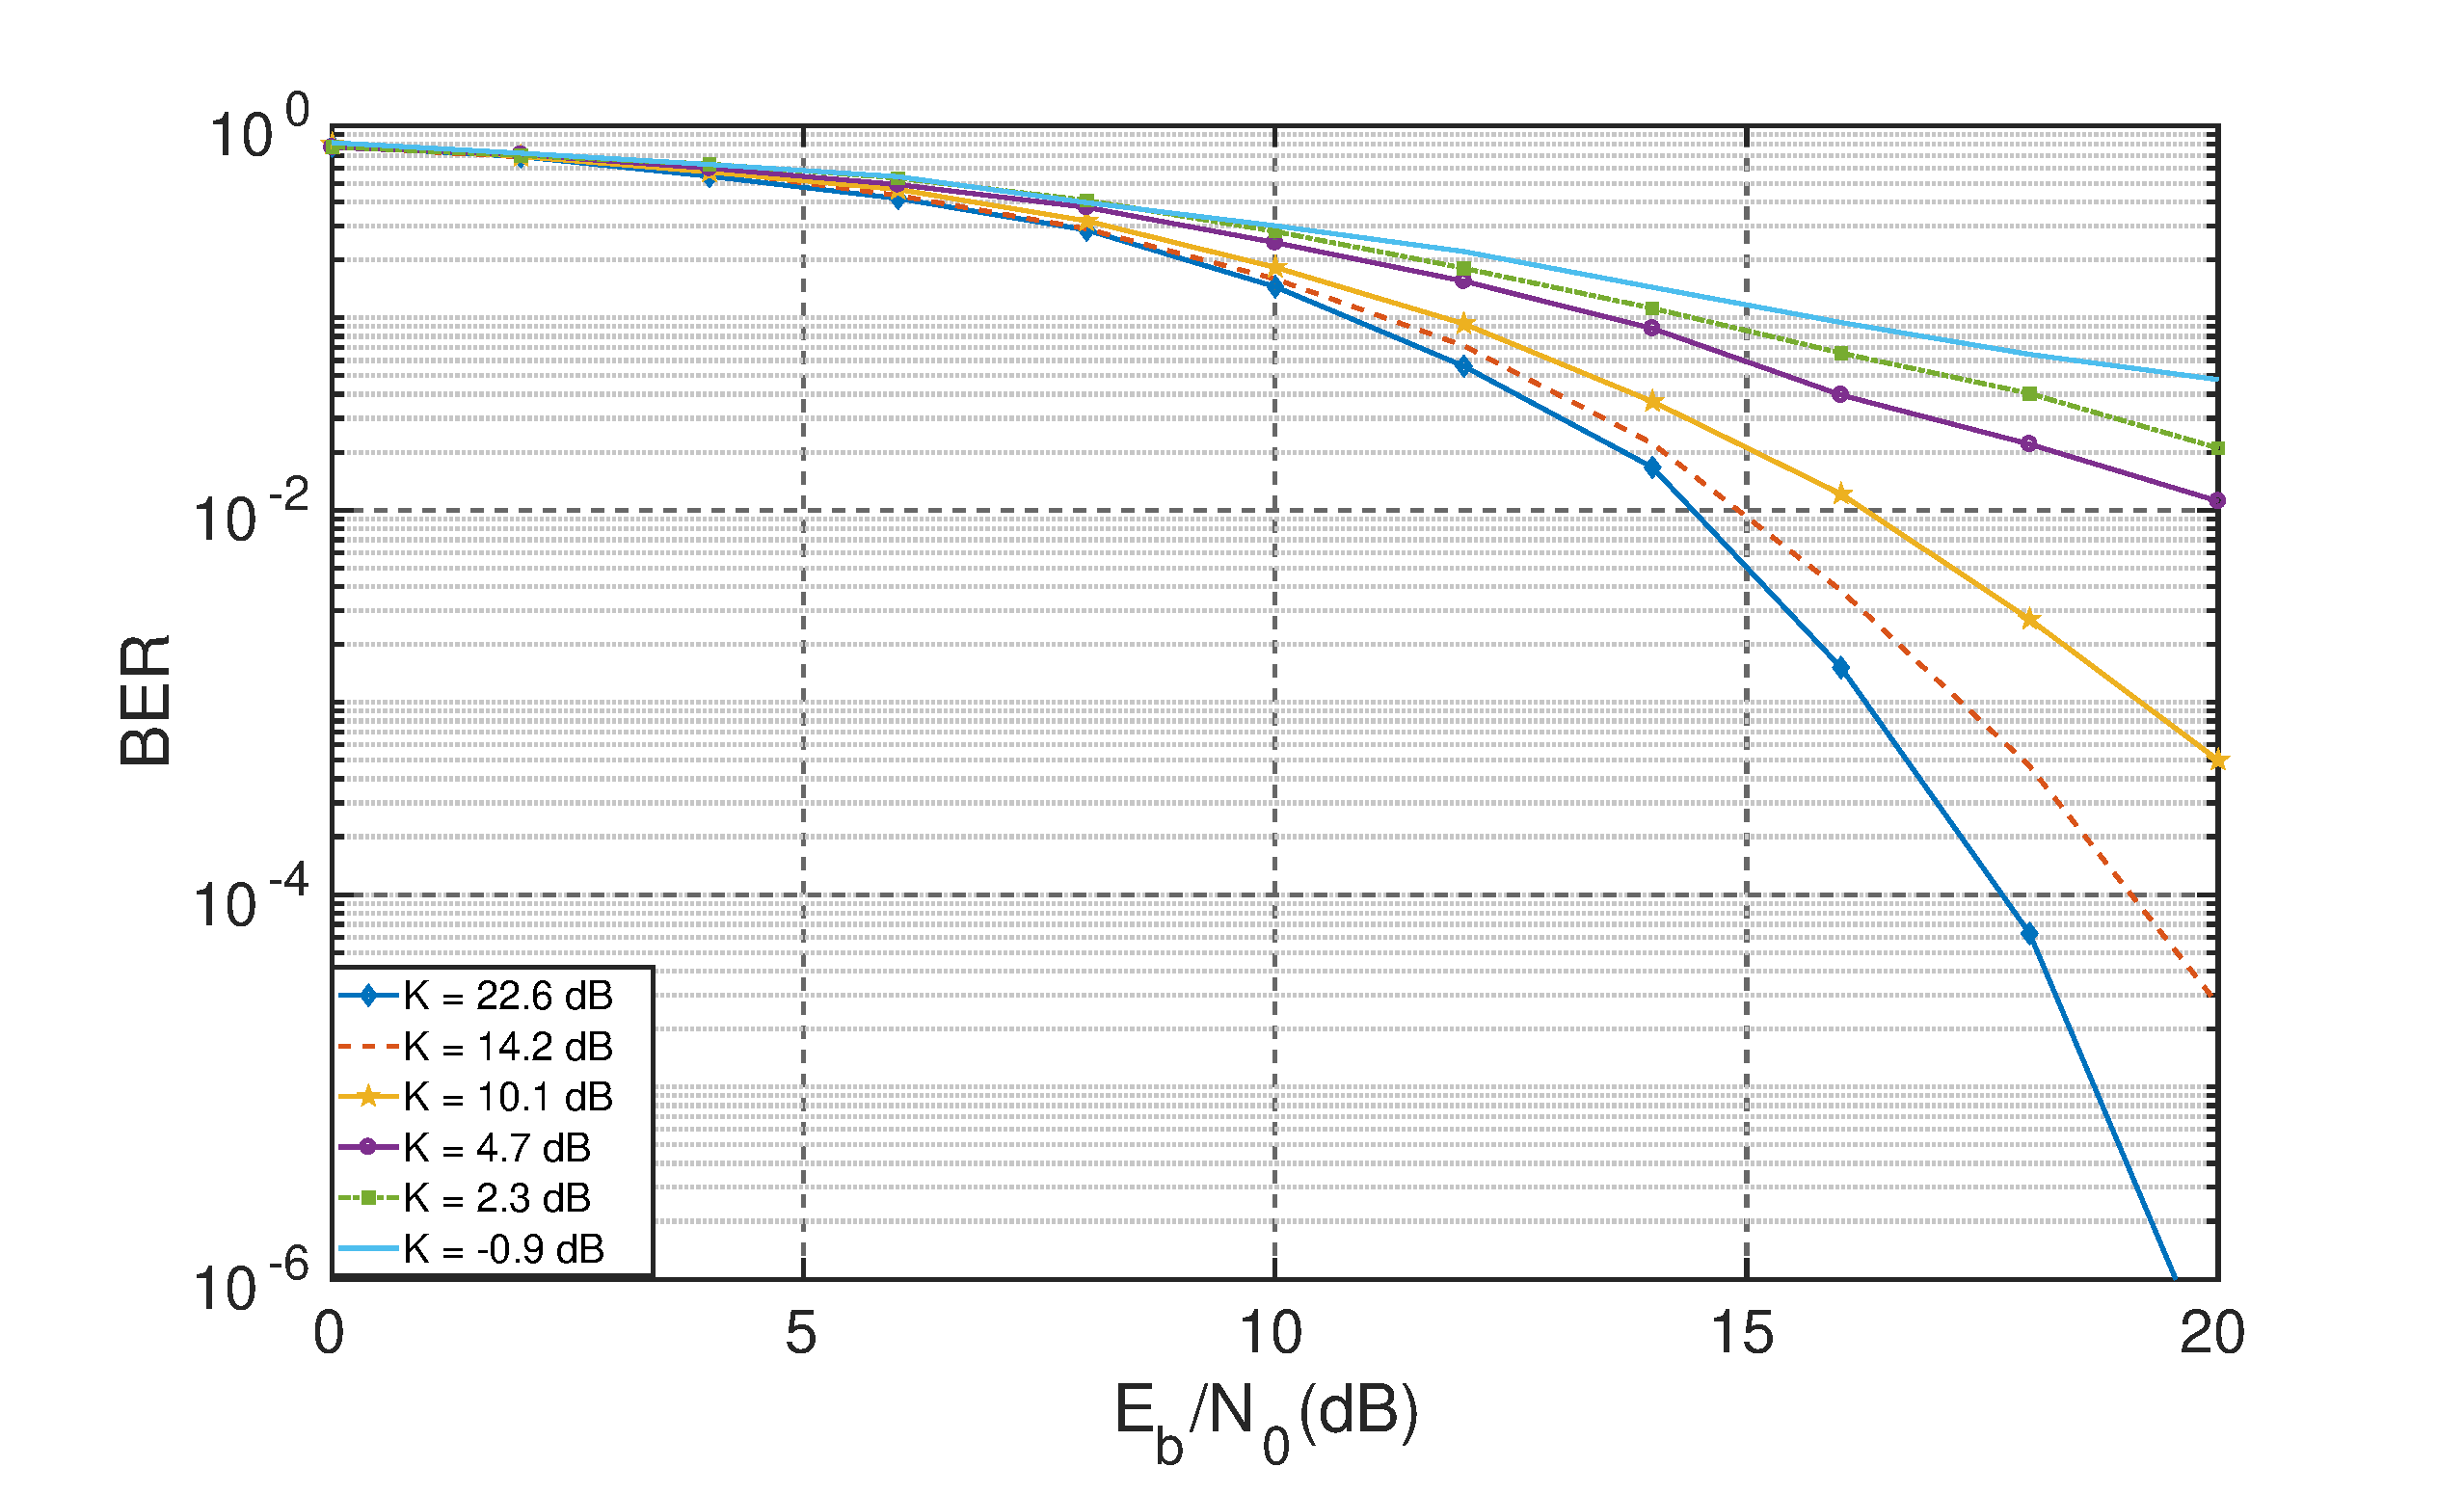
\includegraphics[width=0.46\textwidth]{images/Gill/lte_figs/64qamricean.eps}}\hspace{1mm}
   \subfloat[OFDM-MQAM]{\label{fig:qamall}\includegraphics[width=0.46\textwidth]{images/Gill/lte_figs/mqamricean.eps}}\hspace{1mm}
     \caption{Comparison of $E_b/N_0$ verus BER for LTE-R OFDM modulation with different $K$-factors. The first three sub-figures shows the $E_b/N_0$ versus BER for individual modulation schemes employed in LTE-R and in last plot we compare all the modulation schemes for different $K$-factors.} 
\label{fig:modulation}      
   \end{center}
\end{figure*}

In Fig.~\ref{kfactorber} we calculate the BER performance for a high speed train in discrete time-steps. As the train moves towards
the LCX slot the SNR goes high and the SNR decreases as the train moves away. This trend can be seen in the plot, as we move towards the slot the BER curve decreases and it starts increases once we move. It is important to consider here that due to the varying nature of K-factor the BER curve also varies significantly. Hence, by considering the time-varying nature of K-factor we can have a better performance analysis.

\begin{figure}[!ht]
\label{kfactorber}
\centering
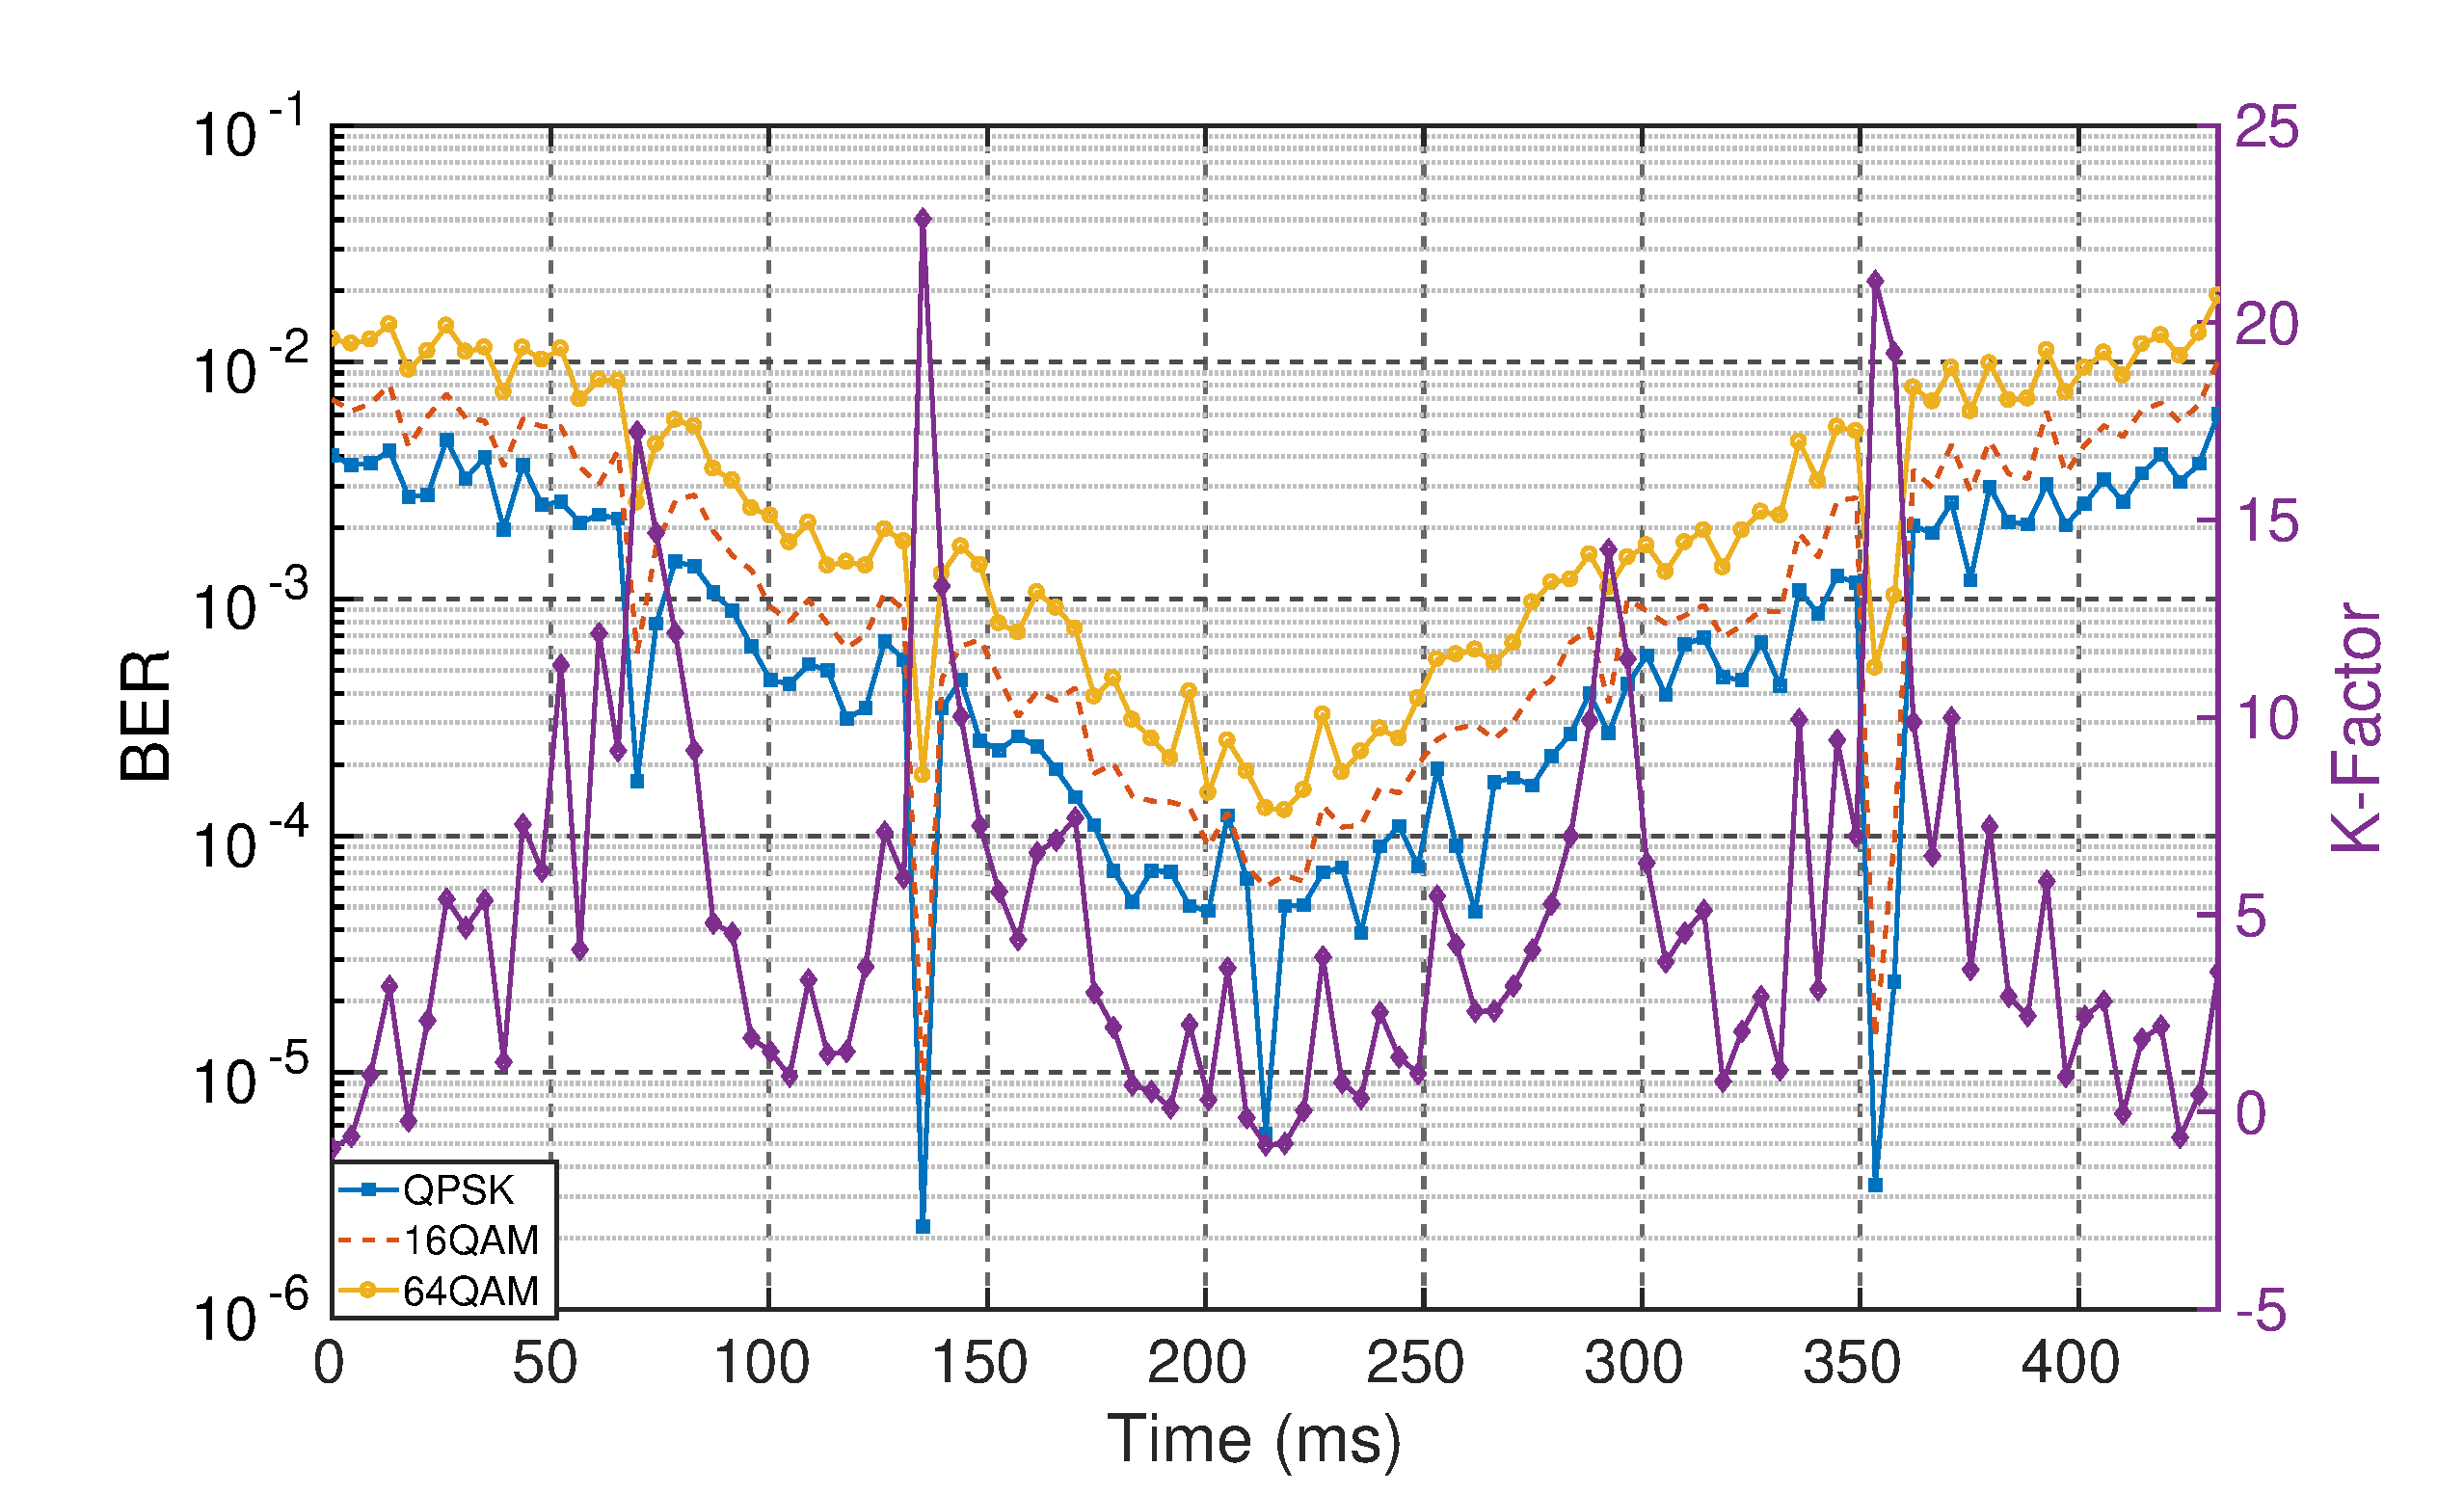
\includegraphics[width=\textwidth,keepaspectratio]{images/Gill/lte_figs/kfactorcontinuous.eps} 
\caption{BER variation with time for HST with different modulation schemes of LTE-R. As the train moves towards
the antenna the general trend of BER goes down with small-scale fluctuations due to varying K-factor.}
\end{figure}


\section{Channel Impairements Inside a Tunnel}
The tunnel environment is affected by multipath and diffraction effects due to multiple reflections from the tunnel walls, which leads to a substantial fading environment. By deploying LCX cables, we can eliminate the large penetration loss due to tunnel walls. However, small-scale fading can still cause a large amount of errors and decrease the QoS for the communication link. High velocity trains experience very high Doppler shifts and a fast fading channel. These problems can lead to significant BER degradation of the LTE system. The frequency shifts caused by the Doppler phenomenon can lead to shifts in the sub-carrier frequencies for OFDM, which leads to synchronization errors. The maximum Doppler shifts for a train traveling at 500 km/h is 2.314 kHz for a 5 GHz carrier frequency. This large Doppler shift can also lead to significant drops in the quality of wireless signals and increase the bit error rate. Thus,
to develop an efficient and reliable communication link inside tunnels, we need to properly model this channel impairment and build our proposed channel model by taking into account these tunnel phenomenons. These impairments are described in detail in the following subsections.

\subsection{Multipath Fading}
The following time-varying multipath channel impulse response considers the effects of Doppler shift and scattering~\cite{booklter13}:
\begin{equation}
\label{channel}
{h}(\tau,t)= \sum_{k=0}^{L}{h_k}(t)e^{-j2\pi f_c\tau_k(t)}\delta[\tau-\tau_k(t)],
\end{equation}
where $\tau$ is the path delay, $t$ is time in seconds, $\delta[\tau-\tau_k(t)]$ is the impulse response, $f_c$ is the carrier frequency, $h_k(t)$ is the envelope of the time-varying channel and consists of both large and small-scale fading components. Since the structure of LCX is almost the same as a leaky waveguide, the large scale fading of channel can be modeled linearly~\cite{arlter10}. There is also no signal shadowing and the line-of-sight (LOS) signal component is always present along the tunnel. This type of channel fading can be best described by a Ricean fading model. The probability density function $p(\alpha)$ of a Rician fading model is given by~\cite{inplter12}:
\begin{equation}
p(\alpha) = \dfrac{2\alpha(1+K)}{\Omega}I_0\Bigg(2\alpha\sqrt{\dfrac{K+K^2}{\Omega}}\Bigg)e^{\dfrac{-K-\alpha^2(1+K)}{\Omega}},
\end{equation}
where $K$ is the Rician factor and $\alpha$ is the complex amplitude of the channel response function that has a unity second moment, \textit{i.e.}, $\Omega \equiv E[\alpha^2] = 1$.

\subsection{Doppler Shift}
The 3GPP channel model~\cite{trlter14} is used for its Doppler shift profile in high speed railway environment. The measurements obtained for the Doppler frequency shift are implemented for two scenarios. The first scenario is for an open space while the second scenario is for high speed trains. Doppler shift is not taken into consideration. There exists a third scenario for tunnels using multiple antennas. Since the slots of LCX can be modeled as multiple antenna system, we use this Doppler shift profile for our proposed channel. The Doppler shift variation $f_s(t)$ is described by:

\begin{equation}
\label{eq1}
f_s(t) = f_d\cos\theta(t),
\end{equation}
where \textrm{$f_d$} is the maximum Doppler shift, $\theta$ is the elevation angle and $\cos \theta(t)$ is given by:
\begin{equation}
\cos\theta(t) = 
\left\{
	\begin{aligned}
	 & \dfrac{D_s/2-vt}{\sqrt{\mathrm{D_{min}}^2+\bigg((D_s/2)-vt\bigg)^2}},0\leq t\leq\dfrac{D_s}{v}\\
	 & \dfrac{-1.5D_s+vt}{\sqrt{\mathrm{D_{min}}^2+\bigg((-1.5D_s)-vt\bigg)^2}},\dfrac{D_s}{v}\leq t \leq \dfrac{2D_s}{v}\\
 	\end{aligned}
\right.
\end{equation}
where $D_s/2$ is the initial distance of the train from base-station, and $\mathrm{D_{min}}$ is base-station (BS)-Railway track distance, both in meters; $v$ is the velocity of the train in \textrm{m/s}, $t$ is time in seconds.

\begin{figure}[!ht]
\label{doppler}
\centering
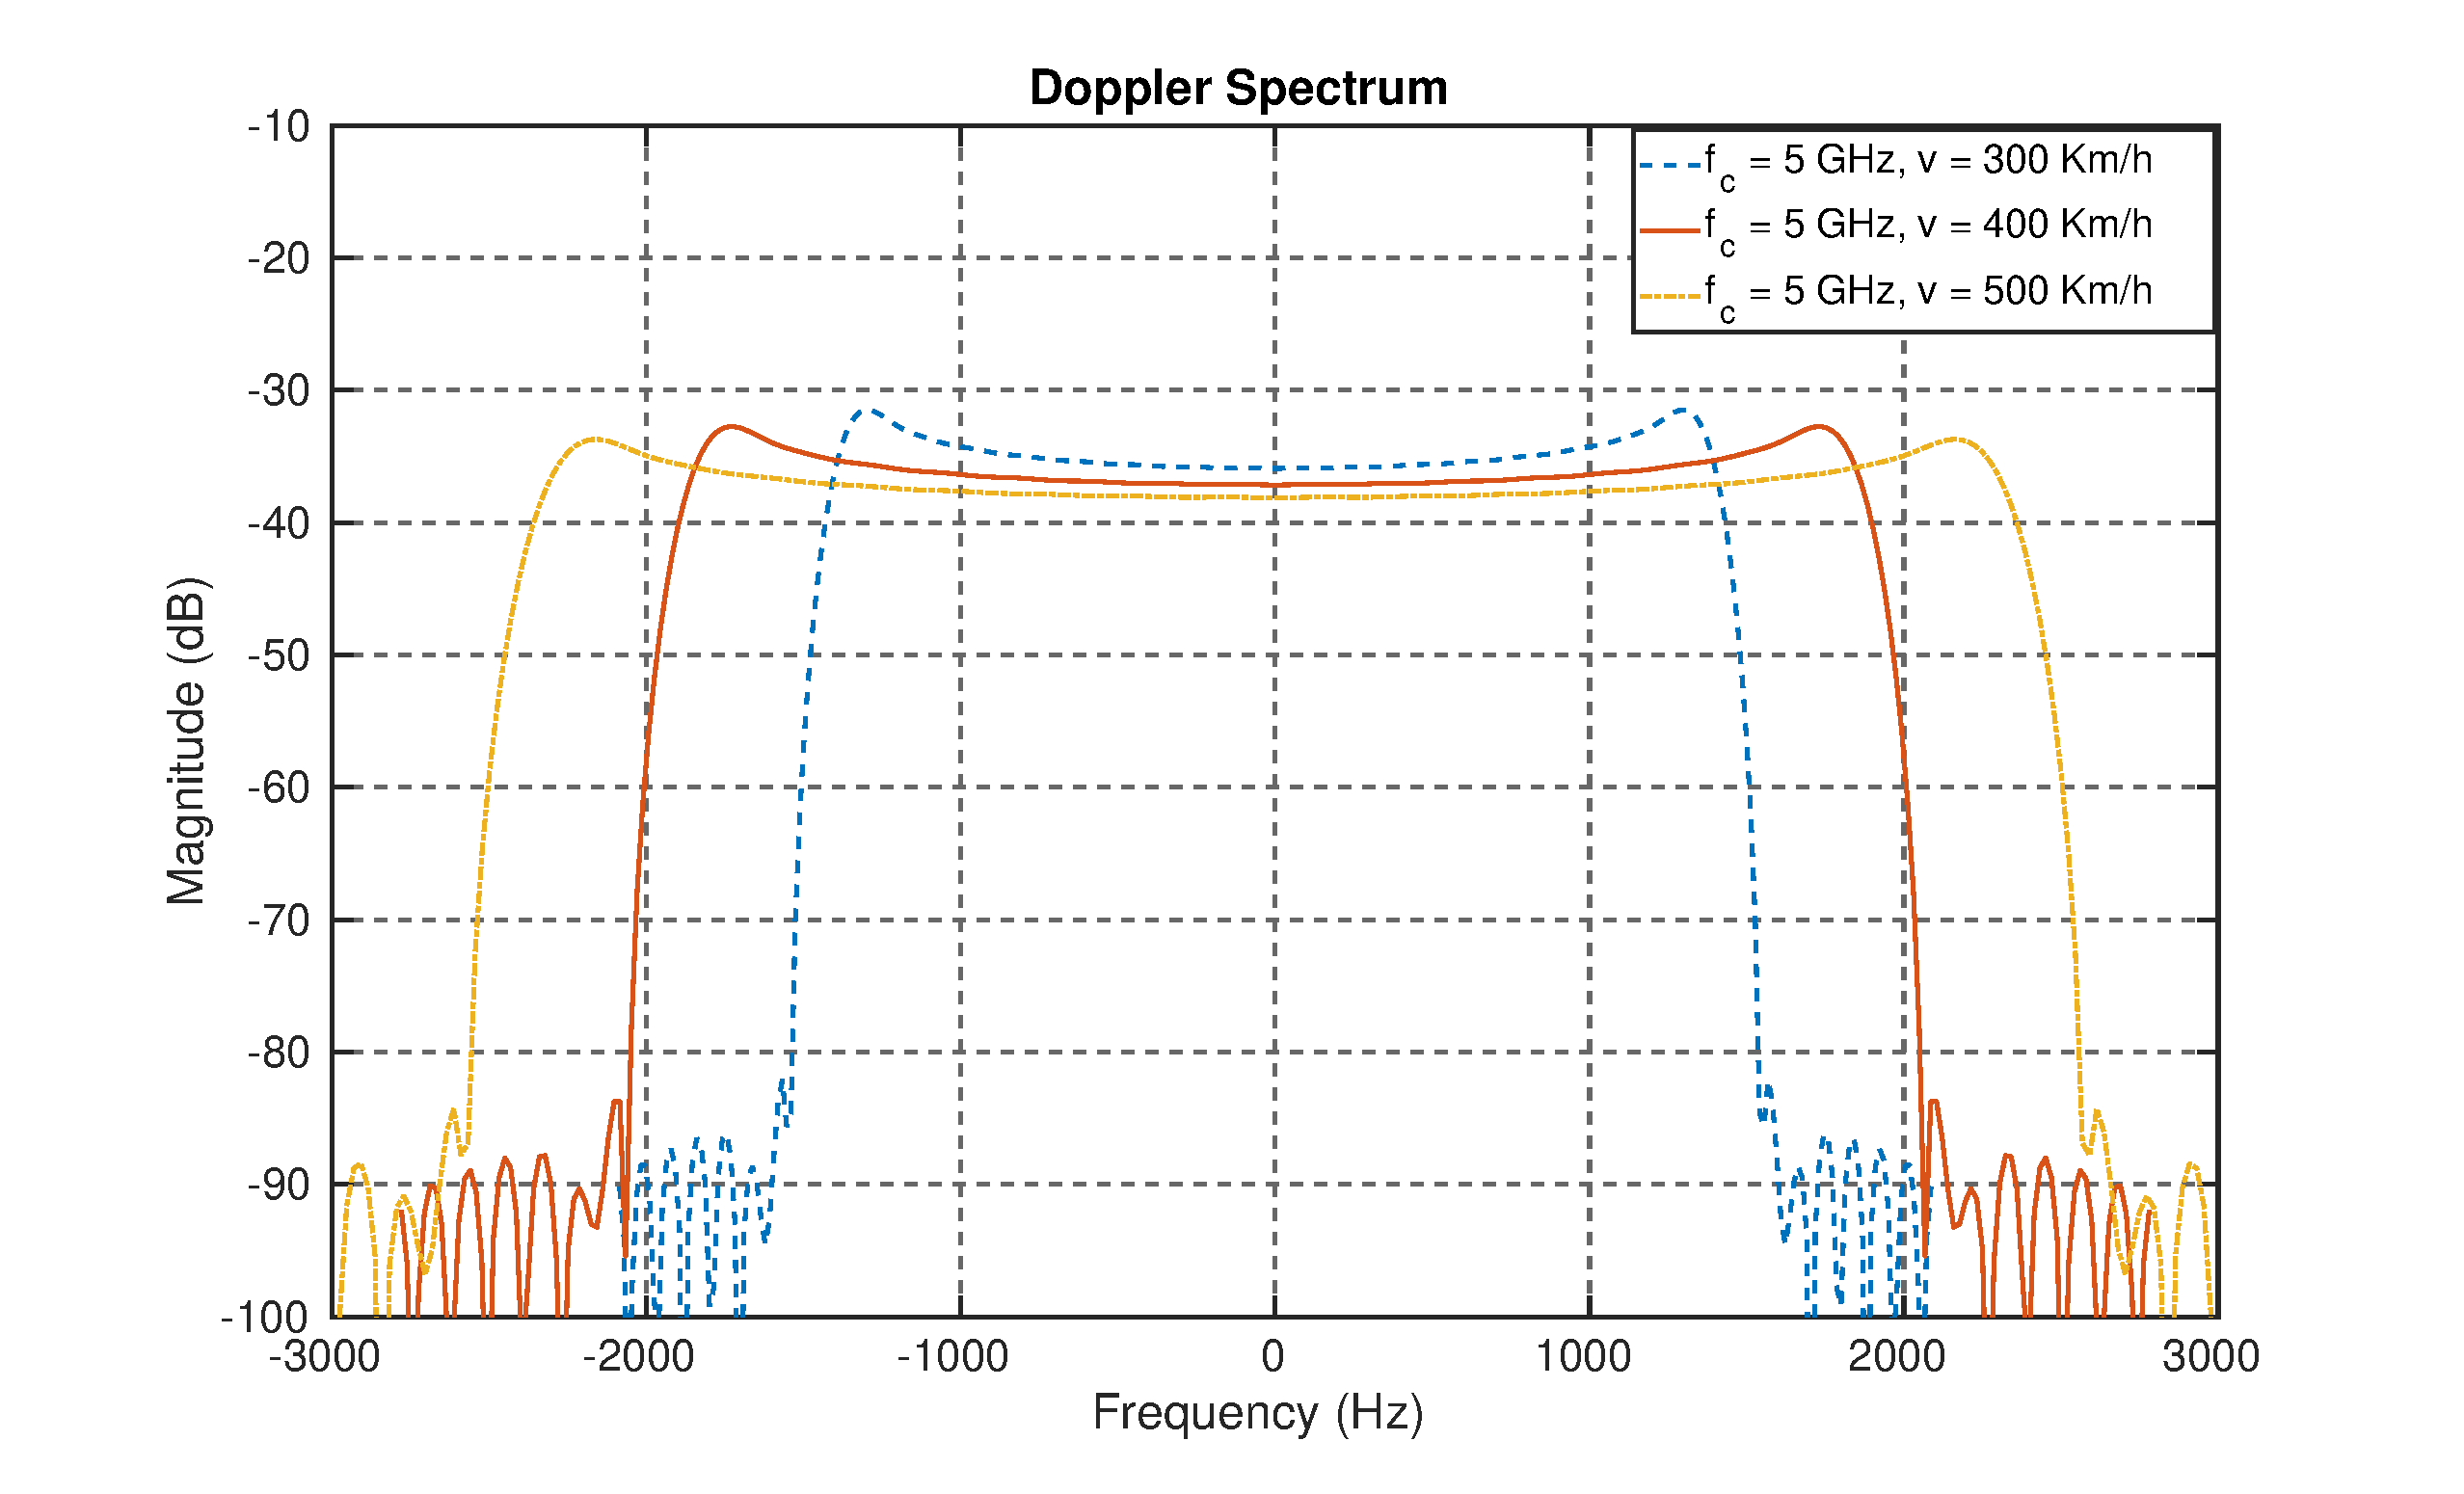
\includegraphics[width=\textwidth,keepaspectratio]{images/Gill/lte_figs/dopplerspectrum.eps} 
\caption{Doppler spectrum for LTE-R at different train velocities $v$ (km/h) = 300, 400 and 500 and $f_c$ = 5 GHz.}
\end{figure}

Figure~\ref{doppler} shows the Doppler spectrum for $f_c$ = 5 GHz and $v$ = 300 Km/h, 400 Km/h and 500 Km/h, and as we can see in the figure the maximum Doppler shift range is from -2.314 kHz to +2.314 kHz. These range of Doppler shift values can lead to very high bit-error rate and poor connectivity in communication system. In the following section we discuss our proposed channel model which consists of Doppler shift profile for high speed train and dynamic K-factor for tunnel environment.

\section{Proposed Channel Model}

The tunnel measurement campaign conducted in~\cite{inplter8} shows that the amplitude variation inside tunnel follows Rician distribution. In the thesis, we apply the approach used in~\cite{inlter15} for single elevation angle $\theta$ and expand it to a time-varying case. In this thesis, we model $\theta$ as a function of time and derive time-series $K$-factor for the tunnel environment. Figure~\ref{subblock} describes our proposed channel model which is implemented using dynamic K-factor and Doppler shift profile derived using Eq.(\ref{eq1}).  In the following section we discuss the classical two-ray propagation model and mathematical derivation of dynamic K-factor for our proposed channel model.

\begin{figure}[!ht]
\label{subblock}
\centering
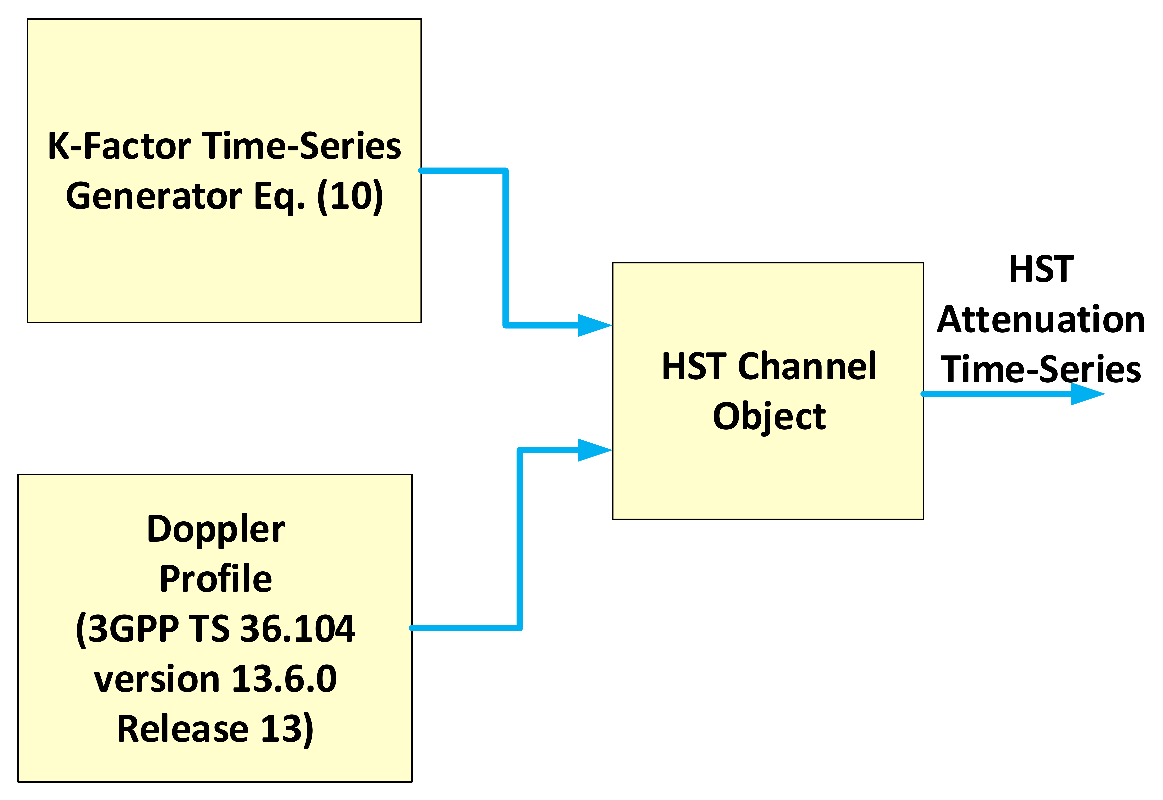
\includegraphics[width=\textwidth,height=6cm,keepaspectratio]{images/Gill/lte_figs/subblock.eps} 
\caption{HST channel model consisting of time-series K-factor and Doppler shift caused due to velocity of the train.}
\end{figure}

The reflection coefficient $\Gamma$~\cite{booklter16} as a function of time $t$ is given by:
\begin{equation}
\Gamma(t) = \dfrac{C\sin\theta(t)-\sqrt{(\varepsilon_r-j\chi(t))-(\cos\theta(t))^2}}{C\sin\theta(t)-\sqrt{(\varepsilon_r-j\chi(t))-(\cos\theta(t))^2}},
\end{equation}
where $C = 1$ is for horizontal polarization, and $C = \varepsilon_r-j\chi(t)$ for vertical polarization. Furthermore, $\chi(t)$ is given by:
\begin{equation}
\chi(t) = \dfrac{\sigma}{\omega(t)\varepsilon_0} = \dfrac{\sigma}{2\pi f_r(t) \varepsilon_0} = \dfrac{1.8\times 10^{10}\sigma}{f_r(t)}.
\end{equation}
with $\varepsilon_0 = 8.854\times 10^{-12}~\textrm{F/m}$, and $\sigma$ is conductivity of the tunnel. The frequency $f_r(t)$ is the resultant frequency caused by the Doppler shift and is given by:
\begin{equation}
f_r(t) = f_c(t)-f_s(t)
\end{equation}
where $f_c(t)$ is the sub-carrier frequency, and $f_s(t)$ is the Doppler shift given by Eq.~(\ref{eq1}).

The phase difference function of $t$, $\Delta\phi(t)$ between the two reflected paths is given by~\cite{booklter11}:
\begin{equation}
\begin{split}
\Delta\phi(t) =& \dfrac{2\pi}{\lambda(t)}\bigg(\sqrt{D_{\textrm{LOS}}^2+(h_t+h_r)^2}-\\
& \sqrt{D_{\textrm{LOS}}^2+(h_t-h_r)^2}\bigg),
\end{split}
\end{equation}
where $\lambda(t)$ is the resultant time-varying wavelength at the receiver, $D_{\textrm{LOS}}$ is the distance between the transmitter and receiver antennas which is changing dynamically with $t$, and both $h_t$ and $h_r$ are the heights of the transmitter and receiver antennas, respectively.
 
The resultant received power $p_r(t)$ is given by the sum of the LOS received power plus the received multipath power, resulting in:
\begin{equation}
\begin{split}
p_r(t) =& ~p_t(t)\bigg(\dfrac{\lambda}{4\pi d}\bigg)^2G_t G_r\bigg[1+\\
& |\Gamma(t)|^2+2|\Gamma(t)|\cos(\angle\Gamma(t)-\angle\Delta\phi(t))\bigg]
\end{split}
\end{equation}
which is a function of the transmitter power $p_t(t)$ and the reflection coefficient $\Gamma(t)$, where $G_t$ and $G_r$ are the transmitter and receiver antenna gains,  respectively.
The $K$-factor is defined as the ratio of the direct path power and the power in the scattered paths, and is given as:
\begin{equation}
\label{kfactor}
\mathrm{K}(t) = \dfrac{1}{|\Gamma(t)|^2+2|\Gamma(t)|\textrm{cos}(\angle \Gamma(t)-\Gamma(t)\Delta\Phi(t))}
\end{equation}

\section{Summary}
We analyzed the BER performance of a LTE-R system for high speed trains inside tunnel environments using our proposed channel model. For the implementation
of our channel, we first derived the time-series K-factor function using the classical two-ray propagation model. We then analyzed the LTE-R performance under our channel model for different modulation schemes for various K-factors. Finally, we compared all the modulation schemes under worst and best K-factor, and we observed that for low $E_b/N_0$
sub-carriers must be modulated with QPSK for maintaining reliable communication link.

